\documentclass[a4paper,11pt]{article}
\usepackage[utf8]{inputenc}
\usepackage[portuguese]{babel}
\usepackage{graphicx}
\usepackage[margin=3cm]{geometry}
\usepackage{subfigmat}

\begin{document}

Tendo o rato a funcionar corretamente, i.e., o cursor a deslocar-se no ecrã refletindo o deslocamento físico do sensor, pede-se que se represente no ecrã do computador a imagem captada pelo sensor. Do \emph{datasheet} lê-se que o registo \texttt{0x0b} do sensor se denomina \emph{pixel-grabber} e que captura um \emph{pixel} por \emph{frame}. Quando este registo é lido e contém um valor válido da intensidade luminosa de um \emph{pixel}\footnote{O sensor apenas capta intensidade luminosa e não uma cor RGB} o MSB é \texttt{1} (bit de validade) e o contador interno é incrementado, fazendo com que na leitura seguinte seja lido o \emph{pixel} com o índice seguinte. Note-se que apenas é capturado um \emph{pixel} por \emph{frame}, portanto não é possível obter um \emph{frame} completo e representá-lo no ecrã. Não obstante como os \emph{frames} consecutivos deverão ser semelhantes a imagem obtida parecerá o resultado de uma só captura. O \emph{datasheet} menciona ainda que qualquer operação de escrita neste registo repõe o contador a zero.

A resolução do sensor do rato é 15 \emph{pixels} por 15 \emph{pixels} totalizando 225 \emph{pixels} que formam a imagem captada pelo sensor. Tendo em conta que só é possível ler a informação relativa a um \emph{pixel} de cada vez, são necessárias 225 leituras para obter a imagem completa.

Para o protocolo de comunicação com o PIC definiu-se que os primeiros 3 \emph{bytes} do pacote são \emph{bytes} de controlo sendo que, do \emph{byte} 0 ao \emph{byte} 2 os seus significados são: a comunicação consiste numa leitura ou numa escrita; o tamanho dos dados comunicados do PIC de volta ao computador; o registo de destino da operação. No caso da operação ser uma escrita, o quarto \emph{byte} corresponde ao conteúdo a escrever no registo de destino. O segundo \emph{byte} de controlo pode especificar ainda uma terceira operação que corresponde à leitura dos \emph{pixels} remanescentes concatenados com as leituras realizadas dos registos do sensor que são os deslocamentos em $xx$ e em $yy$ do rato desde a última leitura.

Para se obterem todos os valores correspondentes aos \emph{pixels} captados pelo sensor são necessárias pelo menos quatro comunicações com o PIC: $$\left\lceil\frac{225}{64-3}\right\rceil=4.$$ Para efeitos de maximização do desempenho decidiu-se realizar quatro e apenas quatro comunicações com o PIC para obter todos os dados necessários para mover o cursor e representar a imagem captada pelo sensor durante um ciclo do programa. Na primeira comunicação obtêm-se os primeiros 61 \emph{pixels}, na segunda comunicação obtém-se do 62º ao 122º \emph{pixels}, na terceira do 123º ao 183º \emph{pixels} e na quarta comunicação obtêm-se os restantes. A figura \ref{pixels} ilustra a correspondência entre os índices dos \emph{pixels} e as suas posições na grelha cartesiana.

\begin{figure}[htb]
	\centering
	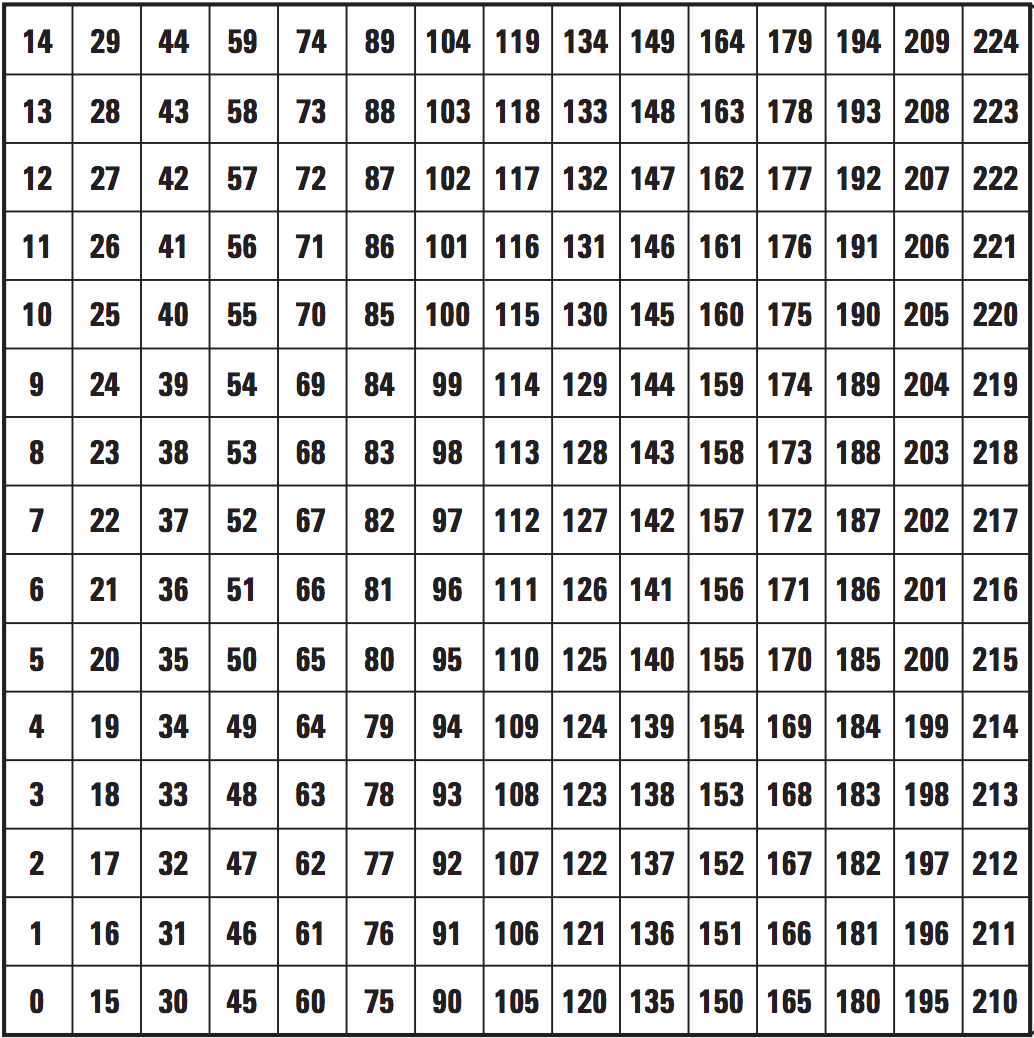
\includegraphics[width=.5\linewidth]{pixels.png}
	\caption{Correspondência entre os índices dos \emph{pixels} e as suas posições na grelha cartesiana.}
	\label{pixels}
\end{figure} 

Para desenhar a imagem captada pelo sensor no ecrã com base nos valores da intensidade luminosa associados a cada pixel utilizaram-se funções da biblioteca \texttt{gdi32} do Windows. Adaptou-se o código fornecido que utiliza esta API para desenhar um retângulo no ecrã para desenhar uma matriz de quadrados de cores diferentes em que cada quadrado corresponde a um \emph{pixel} captado pelo sensor. O código resultante lista-se abaixo.

\begin{verbatim}

#define SCALE 15

HDC hdcScreen = GetDC(NULL);
HDC MemDCExercising = CreateCompatibleDC(hdcScreen);
HBITMAP bm = CreateCompatibleBitmap(hdcScreen, 15 * SCALE, 15 * SCALE);
SelectObject(MemDCExercising, bm);

HBRUSH hBrush;
HPEN hPen;
	
/* image is a vector that contains the values that refer to the luminosity
of the pixels */
for(int i = 0; i < 225; i++)
{
int x = i / 15;
int y = 14 - (i % 15);
int color = image[i];

hBrush = CreateSolidBrush(RGB(color, color, color));
SelectObject(MemDCExercising, hBrush);
hPen = CreatePen(PS_SOLID, 1, RGB(color, color, color));
SelectObject(MemDCExercising, hPen);
Rectangle(MemDCExercising, x*SCALE, y*SCALE, (x+1)*SCALE, (y+1)*SCALE);
DeleteObject(hBrush);
DeleteObject(hPen);
}
	
BitBlt(hdcScreen, 0, 0, 15*SCALE, 15*SCALE, MemDCExercising, 0, 0, SRCCOPY);
DeleteObject(bm);
DeleteDC(MemDCExercising);

\end{verbatim}

A título de exemplo capturaram-se dois fotogramas da imagem capturada pelo sensor do rato e representada no ecrã. Estes resultados ilustram-se na imagem \ref{samples}.

\begin{figure}
	\begin{subfigmatrix}{2}
		\subfigure[Amostra 1]{
\includegraphics[width=.3\linewidth]{sample1.png}}
		\subfigure[Amostra 2]{
\includegraphics[width=.3\linewidth]{sample2.png}}
	\end{subfigmatrix}
	\caption{Imagens capturada pelo sensor do rato e representadas no ecrã.}
	\label{samples}
\end{figure}

\end{document}